% !TEX program = xelatex
%\documentclass[notes=show]{beamer}
\documentclass[notes=hide]{beamer}
%\documentclass[notes=onlyslideswithnotes,notes=hide]{beamer}
%\documentclass[notes=only]{beamer}
%\documentclass[11pt,letterpaper]{article}
%\usepackage{beamerarticle}

\usepackage{genchem}
\usepackage{lecture}
\usepackage{multicol}
\usepackage{elements}
\usepackage{collcell}
\usetikzlibrary{tikzmark}
\usepackage{tabularx}
\usepackage{ccicons}

\title{Liquids, Solids, and Intermolecular Forces}
\subtitle{Chapter 11}
\institute[CHEM115 Bloomsburg University]{CHEM115 --- Chemistry for the Sciences I \\ Bloomsburg University}
\author{D.A. McCurry}
\date{Fall 2020}

\chemsetup{chemformula/frac-style=nicefrac}

\begin{document}

\maketitle
\mode<article>{\thispagestyle{fancy}}

\frame{\section{States of Matter and IMF}
	\begin{learningobjectives}
	\item Explain why different states of matter occur.
	\item Compare the types of intermolecular forces (IMF).
	\item Predict all of the IMF present between certain molecules.
	\end{learningobjectives}
}

\begin{frame}{Structure Determines Properties}
	\only<+>{%
	\begin{itemize}
		\item The chemical composition and the molecular structure of
			chemical species determine the type and overall strength
			of its \alert{intermolecular forces}.
			\begin{block}{Intermolecular Forces (IMF)}
				The attractive forces that exist \alert{between} all molecules
				and atoms.
			\end{block}

		\item Intermolecular forces hold liquids and solids together.
			\begin{itemize}
				\item They are responsible for the very
					existence of condensed states/phases of
					matter.
			\end{itemize}

		\item The phases of matter (e.g., solid, liquid, or gas) depend
			on the \alert{magnitude} of the intermolecular forces between
			the constituent particles, relative to the amount of
			thermal energy.
	\end{itemize}
}

\only<+>{%
	\begin{center}
		\includegraphics[scale=0.45]{11_Pg473_UnTable.jpg}
	\end{center}
}
\end{frame}

\clearpage

\begin{frame}{The Phases of Matter}
	\only<+>{%
	\begin{center}
		\includegraphics[scale=0.4]{11_01_Table.jpg}
	\end{center}
}

\only<+>{%
	\begin{center}
		\includegraphics[scale=0.45]{11_Pg466_UnFigure_1.jpg}
	\end{center}

	\begin{tabularx}{\linewidth} {l l l l >{\raggedright\arraybackslash}X}
		\toprule
		\textbf{State} & \textbf{Density} & \textbf{Shape} &
		\textbf{Volume} & \textbf{Relative Strength of IMF} \\ \midrule
		Gas & Low & Indefinite & Indefinite & Weak \\
		Liquid & High & Indefinite & Definite & Moderate \\
		Solid & High & Definite & Definite & Strong \\ \bottomrule
	\end{tabularx}
}
\end{frame}

\vspace{\stretch{-1}}

\begin{frame}{Gases}
	\begin{itemize}
		\item Gas particles have complete freedom of motion, constantly
			moving around in a random pattern, but not ``sticking''
			to each other.
		\item There is a large amount of space between gas particles.
			\begin{itemize}
				\item Gases are compressible.
			\end{itemize}
	\end{itemize}

	\begin{center}
		\includegraphics[scale=0.35]{11_02_Figure.jpg}
	\end{center}
\end{frame}

\vspace{\stretch{-1}}

\begin{frame}{Liquids}
	\begin{columns}
		\column{0.5\textwidth}
		\begin{itemize}
			\item The particles in a liquid are closely packed, but
				they have some ability to move around.
			\item They are free to take the shape of their container
				and flow.
		\end{itemize}
		\column{0.5\textwidth}
		\begin{center}
			\includegraphics[scale=0.4]{11_1_Figure.jpg}
		\end{center}
	\end{columns}
\end{frame}

\vspace{\stretch{-1}}

\begin{frame}{Solids}
	\begin{itemize}
		\item Solid particles are packed close together and are fixed in
			position.
		\item Solids retain their shape and volume when placed in a
			container.
		\item Solid particles are characterized based on their
			\alert{arrangements}:
			\begin{description}
				\item[Crystalline:] Orderly, geometric patterns
					(salts, diamond)
				\item[Amorphous:] Irregular, no regular pattern
					(plastic, glass)
			\end{description}
	\end{itemize}
	
	\begin{center}
		\includegraphics[scale=0.2]{11_03_Figure.jpg}
	\end{center}
\end{frame}

\begin{frame}{Intermolecular Forces}
	\begin{center}
		\includegraphics[scale=0.15]{11_Pg467_UnFigure_1.jpg}
	\end{center}

	\begin{itemize}[<+->]
		\item All attractive forces between particles are electrostatic
			in nature.
			\begin{align*}
				\textbf{Coulomb's Law:} \qquad
				E=\frac{1}{4\pi\epsilon_0} \frac{q_1q_2}{r}
			\end{align*}
		\item The strength of these attractions determines the state
			(solid, liquid, gas) of a substance.
		\item These attractive forces can vary in strength based on the
			composition of the particles.
	\end{itemize}
\end{frame}

\begin{frame}{Dispersion Forces}{or London dispersion forces or van der Waals
	forces}
	\begin{itemize}
		\item Dispersion forces are \alert{weak} attractions between
			molecules.
		\item They are caused by \alert{temporary dipoles} that develop
			when electrons are not distributed equally.
	\end{itemize}

	\bigskip

	\begin{overlayarea}{\linewidth}{12em}
		\begin{center}
			\alt<2->{\includegraphics[scale=0.4,trim={0 0 0
			50pt},clip]{11_04_Figure.jpg}}
			{\includegraphics[scale=0.4]{11_Pg467_UnFigure_2.jpg}}
		\end{center}
	\end{overlayarea}
\end{frame}

\begin{frame}{Effect of Molecular Size on Dispersion Forces}
	\begin{center}
		\includegraphics[scale=0.4]{11_03_Table.jpg}
	\end{center}
\end{frame}

\vspace{\stretch{-1}}

%\mode<article>{\clearpage}

\begin{frame}{Effect of Molecular Shape on Dispersion Forces}
	\only<+>{%
	\begin{center}
		\includegraphics[scale=0.3]{11_Pg468_UnFigure.jpg}

		\includegraphics[scale=0.3]{11_05_Figure.jpg}
	\end{center}
}

\only<+>{%
	\begin{center}
		\includegraphics[scale=0.45]{11_06_Figure.jpg}
	\end{center}
}
\end{frame}

\vspace{\stretch{-1}}

\begin{frame}{Dipole-Dipole Forces}
	In \alert{polar} molecules, electron-rich regions (with a partial
	positive charge) are attracted to electron-poor regions (with a partial
	negative charge).

	\bigskip

	\begin{overlayarea}{\linewidth}{15em}
	\alt<2->{
		Due to the \alert{permanent} nature of the dipoles, these forces are
		\alert{much stronger} than dispersion forces.
	
		\begin{center}
			\includegraphics[scale=0.4]{11_Pg470_UnTable.jpg}
		\end{center}
	}{
		\begin{center}
			\includegraphics[scale=0.4,trim={0 0 0 40pt},clip]{11_07_Figure.jpg}
		\end{center}
	}
	\end{overlayarea}
\end{frame}

\vspace{\stretch{-1}}

\begin{frame}{Effect of Dipole Moment on Boiling Point}
	\begin{center}
		\includegraphics[scale=0.4]{11_08_Figure.jpg}
	\end{center}
\end{frame}

\vspace{\stretch{-1}}

\begin{frame}{Effect of Dipole-Dipole Forces on Miscibility}{The ability to mix
	without separating into two states.}

	\begin{center}
		\includegraphics[scale=0.45]{11_09_Figure.jpg}
	\end{center}
\end{frame}

\vspace{\stretch{-1}}

\begin{frame}{Hydrogen Bonding}
	\only<+>{%
	\alert{Hydrogen bonds} occur between hydrogen atoms bonded to \ch{F},
	\ch{O}, or \ch{N}, and other atoms that are very electronegative.
	\begin{itemize}
		\item The electronegative atom leaves \ch{H} with a very large
			partial postive charge.
	\end{itemize}

	\bigskip

	\begin{center}
		\includegraphics[scale=0.4,trim={0 0 0 50pt},clip]{11_10_Figure.jpg}
	\end{center}
}

\only<+>{%
	\begin{center}
		\includegraphics[scale=0.4]{11_11_Figure.jpg}
	\end{center}
}

\only<+>{%
	\begin{center}
		\includegraphics[scale=0.35]{11_13_Figure.jpg}
	\end{center}
}

\only<+>{%
	\begin{columns}
		\column{0.5\textwidth}
		\begin{center}
			\includegraphics[scale=0.075]{DNA.png}
		\end{center}
		\column{0.5\textwidth}
		\begin{itemize}
			\item Hydrogen bonds are incredibly important in
				biology.
			\item Complementary DNA strands are held together via
				hydrogen bonds, yet they are easily ``unzipped''
				for transcription or replication.
		\end{itemize}
	\end{columns}
}

\only<+>{%
	\begin{center}
		\begin{tikzpicture}
			\node(hbond1) {\includegraphics[scale=1]{hbond-1.png}};
			\node[anchor = north west](hbond2) at ($(hbond1.north east) + (1,0)$)
				{\includegraphics[scale=1]{hbond-2.png}};
			\node[below = of hbond2,text width = 0.45\linewidth]{
				Hydrogen bonding in liquid water is \alert{dynamic}.};
		\end{tikzpicture}
	\end{center}
}
\end{frame}

\begin{frame}{Ion-Dipole Forces}
	\begin{itemize}
		\item When ionic compounds are mixed with polar compounds, the
			charges of the ions interact with the polar regions of
			the molecules.
		\item Overall, one of the strongest intermolecular forces.
	\end{itemize}

	\bigskip

	\begin{center}
		\includegraphics[scale=0.4,trim={0 0 0
		210pt},clip]{11_14_Figure.jpg}
	\end{center}
\end{frame}

\begin{frame}{Intermolecular Forces Summary}
	\begin{center}
		\includegraphics[scale=0.4,trim={20pt 20pt 0
		40pt},clip]{11_04_Table.jpg}
	\end{center}
\end{frame}

\clearpage

\begin{frame}{How to Determine the Intermolecular Forces Present}
	\begin{center}
		\fontsize{9.5}{12}\selectfont
		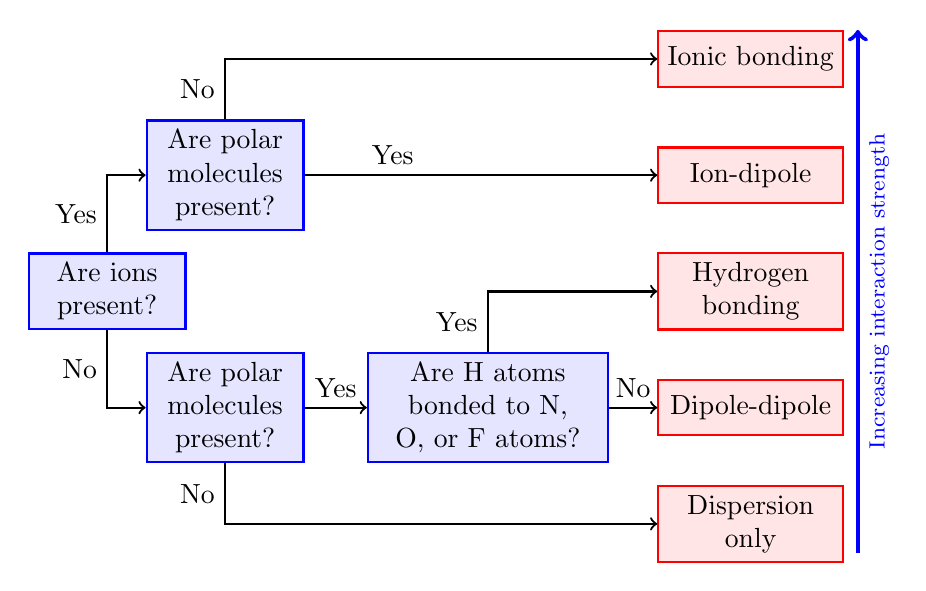
\begin{tikzpicture}[x=7.75em,y=4.2em]
			\tikzstyle{question}=[
				draw=blue,
				thick,
				fill=blue!10,
				align=center,
				text width=5em,
				minimum height=2em,
			%	font=\small
			];
			\tikzstyle{answer}=[draw=red,
				thick,
				fill=red!10,
				align=center,
				text width=6em,
				minimum height=2em,
			%	font=\small
			];
			\tikzstyle{arrow}=[->,thick];
			\node[question](ionic) at (0,0) {Are ions present?};
			\node[question](ionpolar) at (0.55,1) {Are polar molecules present?};
			\node[question](polar) at (0.55,-1) {Are polar molecules present?};
			\node[question,text width=8em](hatoms) at (1.775,-1) {Are \ch{H} atoms bonded to \ch{N}, \ch{O}, or \ch{F} atoms?};
			\node[answer](iondipole) at (3,1) {Ion-dipole};
			\node[answer](ionbonding) at (3,2) {Ionic bonding};
			\node[answer](dispersion) at (3,-2) {Dispersion only};
			\node[answer](dipoledipole) at (3,-1) {Dipole-dipole};
			\node[answer](hbonding) at (3,0) {Hydrogen bonding};
			\draw[arrow] (ionic) |- (ionpolar) node[near start,left] {Yes};
			\draw[arrow] (ionic) |- (polar) node[near start,left] {No};
			\draw[arrow] (ionpolar) -- (iondipole) node[near start,above] {Yes};
			\draw[arrow] (ionpolar) |- (ionbonding) node[near start,left] {No};
			\draw[arrow] (polar) -- (hatoms) node[midway,above] {Yes};
			\draw[arrow] (polar) |- (dispersion) node[near start,left] {No};
			\draw[arrow] (hatoms) -- (dipoledipole) node[midway,above] {No};
			\draw[arrow] (hatoms) |- (hbonding) node[near start,left] {Yes};
			\draw[->,ultra thick,blue] (3.5,-2.25) -- (3.5,2.25) node[midway,below,rotate=90,font=\footnotesize] {Increasing interaction strength};
		\end{tikzpicture}
	\end{center}
\end{frame}

\vspace{\stretch{-1}}

\begin{frame}[t]{Identifying Forces}
	Identify the \textbf{main} type of attractive forces for each compound:

	(ionic, dipole-dipole, hydrogen bonds, or dispersion forces only)

	\bigskip

	\begin{enumerate}
		\item \ch{NCl3} \note<1>[item]{dipole-dipole}
		\item \ch{H2O}  \note<1>[item]{hydrogen bonds}
		\item \ch{Br2}  \note<1>[item]{dispersion}
		\item \ch{KCl}  \note<1>[item]{ionic}
		\item \ch{NH3}  \note<1>[item]{hydrogen bonds}
	\end{enumerate}

	\pause

	\bigskip

	Rank the compounds in order of \textbf{increasing} intermolecular force
	strength.

	\note<2>{
		$ \ch{Br2} < \ch{NCl3} < \ch{NH3} < \ch{H2O} < \ch{KCl} $
	}
\end{frame}

\bigskip

\begin{onyourown}[0em]
	Identify \textbf{all} of the attractive forces for each compound:
	% Ebbing, 8th Ed Problem 11.57

	\bigskip

	\begin{enumerate}
		\item \ch{BF3} \\
		\item isopropyl alcohol, \ch{CH3CHOHCH3} \\
		\item hydrogen iodide, \ch{HI} \\
		\item krypton, \ch{Kr}
	\end{enumerate}
\end{onyourown}



\begin{frame}{Some more biology\ldots}
	\only<+>{%
	\begin{columns}
		\column{0.5\textwidth}
		\begin{itemize}
			\item Amino acids are the building blocks of proteins.
			\item Each different amino acid contains different
				\alert{functional groups} which exhibit different
				interactions.
		\end{itemize}
		\column{0.5\textwidth}
		\begin{center}
			\includegraphics[scale=0.35]{aminoacids.jpg}
		\end{center}
	\end{columns}
}

\only<+>{%
	\begin{center}
		\includegraphics[scale=0.375]{proteinfold.jpg}
	\end{center}
}
\end{frame}

\frame{\section{Intermolecular Forces in Action}
	\begin{learningobjectives}
	\item Identify common phenomena resulting from IMF.
	\item Explain the relationship between energy and IMF.
	\item Calculate the energy required to change the state of compounds.
	\item Identify the phase of a compound from a phase diagram.
	\end{learningobjectives}
}

\vspace{\stretch{-1}}

\begin{frame}{Surface Tension}
	\begin{block}{Surface Tension}
		The energy required to increase the surface area by a unit
		amount.
	\end{block}

	\bigskip

	\begin{columns}
		\column{0.5\textwidth}
		\begin{itemize}[<+->]
			\item It requires energy to ``push'' through substances.
			\item How does this pond skater ``walk'' on water?
			\item Water has a surface tension of
				\SI{72.8}{\milli\joule\per\meter\squared}
		\end{itemize}
		\column{0.5\textwidth}
		\begin{center}
			\begin{tikzpicture}
				\node(bug){\includegraphics[scale=0.1]{Gerris_by_webrunner.JPG}};
				\node[below = 0pt of bug,font=\footnotesize]{\ccbysa\ webrunner};
			\end{tikzpicture}
		\end{center}
	\end{columns}
\end{frame}

\vspace{\stretch{-1}}

\begin{frame}{Viscosity}
	\begin{block}{Viscosity}
		The resistance of a liquid to flow. Measured in poise
		($\SI{1}{P} = \SI{1}{\gram\per\centi\meter\per\second}$).
	\end{block}

	\medskip

	Viscosity increases with\ldots
	\begin{itemize}
		\item increased intermolecular forces.
		\item larger molar mass.
		\item increasing chain length.
	\end{itemize}

	\medskip

	\begin{center}
		\includegraphics[scale=0.35,trim={20pt 20pt 0
		30pt},clip]{11_05_Table.jpg}
	\end{center}
\end{frame}

\vspace{\stretch{-1}}

\begin{frame}[t]{Capillary Action}
	\begin{block}{Capillary Action}
		The ability of a liquid to flow against gravity up a narrow
		tube.
	\end{block}

	\bigskip

	\only<+>{%
	Combines two forces:
	\begin{description}
		\item[Cohesive force:] attraction of molecules in a liquid to
			each other.
		\item[Adhesive force:] attraction of molecules in a liquid to
			the walls of the container.
	\end{description}
}

\only<+>{%
	\begin{center}
		\includegraphics[scale=0.25]{11_18_Figure.jpg}
		\qquad
		\includegraphics[scale=0.25]{11_19_Figure.jpg}
	\end{center}
}
\end{frame}

\begin{frame}{State Changes}
	Recall:\par\medskip\par
	\begin{quote}
		The phases of matter (e.g., solid, liquid, or gas) depend on the
		magnitude of the intermolecular forces between the constituent
		particles, relative to the amount of thermal energy.
	\end{quote}

	\bigskip

	\begin{itemize}[<+(1)->]
		\item A certain amount of energy is required to keep molecules
			close together.
		\item By raising the temperature of a substance, we increase the
			\alert{kinetic energy}.
		\item If the kinetic energy added is strong enough to overcome
			the intermolecular forces, we observe a \alert{change of
			state}.
	\end{itemize}
\end{frame}

\begin{frame}{Vaporization}
	\begin{center}
		\includegraphics[scale=0.2]{11_20_Figure.jpg}
		\qquad
		\includegraphics[scale=0.25]{11_21_Figure.jpg}

		\bigskip

		\begin{tabular} {>{\bfseries}r r@{ → }l}
			Vaporization: & liquid & gas \\
			Condensation: & gas & liquid
		\end{tabular}
	\end{center}

	Compounds that vaporize easily are considered \alert{volatile} whereas
	those that do not are considered \alert{nonvolatile}.
\end{frame}

\begin{frame}{Enthalpy of Vaporization}
	\only<1-3>{%
	In order to vaporize a substance, energy is required:
	\begin{reaction*}
		\water\lqd{} -> \water\gas{}
		"\qquad\enthalpy[subscript-right=vap,superscript-right=]{+40.7}"
	\end{reaction*}
	This energy is known as the \alert{enthalpy of vaporization} or
	\alert{heat of vaporization} and is \alert{always positivie}.

	\onslide<2->

	\bigskip

	What is the enthalpy of the following reaction?
	\begin{reaction*}
		H2O\gas{} -> H2O\lqd{}
	\end{reaction*}

	\onslide<3->

	We can use the heat of vaporization to calculate how much heat is
	needed in order to vaporize an entire mass of a sample.
	}

	\only<4>{%
	
	Are there any observable trends in the following table?

	\bigskip

	\begin{center}
		\includegraphics[scale=0.4]{11_07_Table.jpg}
	\end{center}
}
\end{frame}

\begin{frame}{Vaporization vs Boiling}
	\only<+>{%
		Above any liquid, there exists a \alert{vapor pressure} due to some
		molecules of the liquid entering the gaseous state.
		\begin{center}
			\includegraphics[scale=0.25]{11_22_Figure}
		\end{center}
		There exists a \alert{dynamic equilibrium} where the rate of vaporization
		is equal to the rate of condensation.
		\begin{reaction*}
			H2O\lqd{} <=> H2O\gas{}
		\end{reaction*}
	}

	\only<+>{%
		\begin{center}
			\includegraphics[scale=0.36]{11_24_Figure.jpg}
		\end{center}
	
		If the dynamic equilibrium is disturbed, the system will respond to
		\alert{minimize} the disturbance and \alert{return} to a state of
		equilibrium.
	}	

	\only<+>{%
		When the vapor pressure of the liquid equals the external pressure, the
		liquid is said to have reached its \alert{boiling point}.
	
		\begin{center}
			\begin{tikzpicture}
				\node(boiling)
				{\includegraphics[width=0.4\linewidth,height=15em,keepaspectratio,trim={175pt
				0 0 0},clip]{11_26_Figure.jpg}};
				\node[draw,above = 1em of boiling,font=\tiny,text
				width=0.35\linewidth,align=center] {
				The water vaporizes both at the surface and the
				\alert{interior} of the liquid.};
			\end{tikzpicture}
			\qquad
			\includegraphics[width=0.4\linewidth,height=15em,keepaspectratio]{11_25_Figure.jpg}
		\end{center}
	
		The \alert{normal boiling point} is the temperature at which the vapor
		pressure is equal to \SI{1}{\atm}.
	}
\end{frame}

\begin{frame}{Sublimation}
	A substances does \alert{not} need to be in the liquid state in order to
	transition to the gaseous state.
	\begin{description}
		\item[Sublimation:] The transition of a solid directly to a
			gas.
		\item[Deposition:] The transition of a gas directly to a solid.
	\end{description}

	\medskip

	\begin{center}
		\includegraphics[height=10em,keepaspectratio]{11_30_Figure.jpg}
		\qquad
		\includegraphics[height=10em,keepaspectratio,trim={0
		0 200pt 0},clip]{11_Pg488_UnFigure.jpg}
	\end{center}
\end{frame}

\vspace{\stretch{-1}}

\begin{frame}{Fusion}
	When a substance melts, it \alert{fuses} into a continuous liquid.
	\begin{description}
		\item[Fusion:] The transition of a solid to a liquid.
		\item[Freezing:] The transition of a liquid to a solid.
	\end{description}

	\bigskip

	\begin{center}
		\includegraphics[scale=0.1]{ice-cube.jpg}
	\end{center}
\end{frame}

\vspace{\stretch{-1}}

\begin{frame}{Enthalpies of Sublimation and Fusion}
	Just as with vaporization, changes of state to/from solids involves an
	energy change:
	\begin{align*}
		\textbf{Sublimation:} && \ch{H2O\sld{} &-> H2O\gas{}} &&
		\enthalpy[subscript-right=sub,superscript-right=]{51.1} \\
		\textbf{Fusion:} && \ch{H2O\sld{} &-> H2O\lqd{}} &&
		\enthalpy[subscript-right=fus,superscript-right=]{6.02}
	\end{align*}

	\smallskip

	\begin{center}
		\begin{tikzpicture}
			\node(vapvsfus)
			{\includegraphics[width=0.5\linewidth,trim={0 0 0
			125pt},clip]{11_32_Figure.jpg}};
			\node[left = 1em of vapvsfus,
				draw,
				align=center,
				text width=0.3\linewidth,
				font=\footnotesize
			] {Heats of fusion are significantly less than heats of
			vaporization.};
		\end{tikzpicture}
	\end{center}
\end{frame}

\vspace{\stretch{-1}}

\begin{frame}{The Heating Curve for Water}
	\begin{center}
	\begin{tikzpicture}
		\node(curve) at (0,0)
		{\includegraphics[width=0.95\linewidth]{11_33_Figure.jpg}};
		\node<2->[draw,align=left,text
		width=0.4\linewidth,fill=white,anchor=north west] at (0,-1.5)
		{Temperature \alert{cannot} change during phase changes!};
	\end{tikzpicture}
\end{center}
\end{frame}

\vspace{\stretch{-1}}

\begin{frame}[t]{Practicing Phase Changes}
	How much energy is needed to convert \SI{10.0}{\gram} of liquid ethanol
	($C_s = \SI{2.04}{\joule\per\gram\per\celsius}$) at \SI{37}{\celsius} to
	ethanol vapor ($\Delta H_\text{vap} = \SI{841}{\joule\per\gram}$,
	$T_\text{boiling} = \SI{78}{\celsius}$)?

	\note{\footnotesize
		\begin{enumerate}
			\item To convert to a gas, we need to first heat the
				liquid to its boiling point:
				\begin{align*}
					q = mC_s\Delta T
					&=
					(\SI{10.0}{\gram})(\SI{2.04}{\joule\per\gram\per\celsius})(\SI{78}{\celsius}
					- \SI{37}{\celsius}) \\
					&= \SI{836.4}{\joule}
				\end{align*}
			\item Then we need to vaporize \alert{all} of the liquid
				to gas:
				\begin{align*}
					\Delta H_\text{vap} &= \frac{q}{n} \\
					q &= n \Delta H_\text{vap}
					=
					(\SI{10.0}{\gram})(\SI{841}{\joule\per\gram})
					\\
					&= \SI{8410}{\joule}
				\end{align*}
			\item Finally, sum together heats:
				\begin{align*}
					q_\text{tot} &= q_1 + q_2 \\
					&= \SI{836.4}{\joule} +
					\SI{8410}{\joule} \\
					&= \SI{9246.4}{\joule}
					= \boxed{\SI{9250}{\joule}}
				\end{align*}
		\end{enumerate}
	}
\end{frame}

\clearpage

\begin{onyourown}
	How much energy is needed to convert \SI{3.45}{\gram} of liquid ethanol
	($C_s = \SI{2.04}{\joule\per\gram\per\celsius}$) at \SI{18}{\celsius} to
	ethanol vapor ($\Delta H_\text{vap} = \SI{841}{\joule\per\gram}$,
	$T_\text{boiling} = \SI{78}{\celsius}$)?
\end{onyourown}

\begin{frame}{Phase Diagrams}
	\begin{center}
		\includegraphics<+>[scale=0.4]{11_35_Figure.jpg}
		\includegraphics<+>[scale=0.4]{11_34_Figure.jpg}
		\mode<article>{\clearpage}
		\includegraphics<+->[width=\linewidth]{11_36_Figure.jpg}
	\end{center}

	\pause[\thebeamerpauses]

	What differs between the \ch{I2}/\ch{CO2} phase diagrams and water?
\end{frame}

\begin{frame}{Water is unique!}
	\begin{itemize}
		\item The density of solid water is \alert{less} than the
			density of liquid water.
		\item Water has a very large melting and boiling point
			compared to other Group VI hydrogen-containing
			compounds.
		\item Water is the \alert{only} main-group hydride that
			is a liquid at room temperature.
	\end{itemize}
	\begin{center}
		\begin{tikzpicture}
			\node{\includegraphics[scale=0.28,trim={0 0 0
				100pt},clip]{11_37_Figure.jpg}};
			\node<presentation:2|article:0>[draw,thick,fill=white,font=\Huge,inner
				sep=8pt]{It's all due to
				\alert{structure}.};
		\end{tikzpicture}
	\end{center}
\end{frame}

\clearpage

\begin{frame}[t]{One last practice\ldots}
	Between periods of a hockey game, a Zamboni resurfaces the ice by
	spreading \SI{300.}{\liter} of water at \SI{40.0}{\celsius} across the
	ice rink.  How much energy (in \si{\kilo\joule}) must the water lose as
	it cools to its freezing point and then freezes? The specific heat of
	water is \SI{4.184}{\joule\per\gram\per\celsius} and
	\enthalpy[subscript-right=fus,superscript-right=]{6.01}.

	\textbf{Note:} \SI{300.}{\liter} of water is \SI{2.98e5}{\gram}~\ch{H2O}
	or \SI{1.65e4}{\mole}~\ch{H2O}.

	\note{\footnotesize
		\begin{enumerate}
			\item To convert to a solid, we need to first cool the
				liquid to its freezing point:
				\begin{align*}
					q = mC_s\Delta T
					&=
					(\SI{2.98e5}{\gram})(\SI{4.184}{\joule\per\gram\per\celsius})(\SI{0}{\celsius}
					- \SI{40.0}{\celsius}) \\
					&= \SI{-4.9873e7}{\joule} =
					\SI{-49873}{\kilo\joule}
				\end{align*}
			\item Then we need to freeze \alert{all} of the liquid
				to solid:
				\begin{align*}
					\Delta H_\text{fus} &= \frac{q}{n} \\
					q &= n \Delta H_\text{fus}
					=
					(\SI{1.65e4}{\mole})\underbrace{(\SI{-6.01}{\kilo\joule\per\mole})}_{\mathclap{\ch{H2O\lqd{}
								->
					H2O\sld{}}}}
					= \SI{-99165}{\kilo\joule}
				\end{align*}
			\item Finally, sum together heats:
				\begin{align*}
					q_\text{tot} &= q_1 + q_2
					= \SI{-149038}{\kilo\joule}
					= \boxed{\SI{-1.49e5}{\kilo\joule}}
				\end{align*}
		\end{enumerate}
	}
\end{frame}

\end{document}
